% !TeX program = lualatex
% !TeX TXS-program:compile = txs:///lualatex/[--shell-escape]
\documentclass{article}
\usepackage[paper=graph, ink=blue, seed=931, background=grid, light=raking, sloppiness=.45,wear=.55,grooves=1,angle=slight]{cacography}
\usepackage{amsmath}
\usepackage{pgfplots}
\pgfplotsset{compat=1.17}
\begin{document}
\cacographypage{stains=coffee,props={pen,sheet},edges=spiral,grooves=1}
\section{Cells per view field}
Three slides, each estimated by eye.
\begin{center}
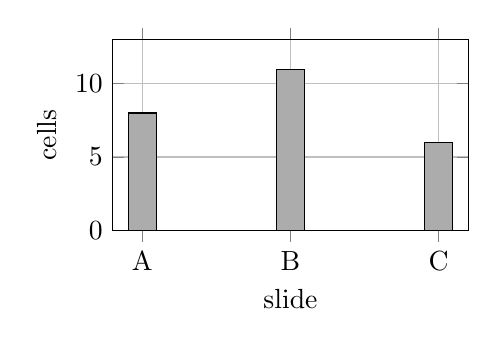
\begin{tikzpicture}
\begin{axis}[width=6.1cm,height=4cm,ybar,bar width=10pt,symbolic x coords={A,B,C},xtick=data,ymin=0,ymax=13,grid=major,xlabel={slide},ylabel={cells}]
\addplot[fill=gray!65] coordinates {(A,8)(B,11)(C,6)};
\end{axis}
\end{tikzpicture}
\end{center}
\cacographynote[right]{repeat blindly}
Slide B seems highest, but selection bias?
\crossout[line]{proof} rough estimate until repeated count.
Clean the objective afterward.
\end{document}
